\documentclass[12pt]{article}
\usepackage{float}
\usepackage[margin=1in]{geometry}
\usepackage[utf8]{inputenc}
\usepackage{footnote}
\usepackage{amsmath,amssymb,graphicx,amsthm}
\usepackage{graphicx}
\usepackage{graphics}
\usepackage{hyperref}
\usepackage{tabularx} % also loads 'array' package
\usepackage{fancyhdr}
\usepackage{lastpage}
\newcolumntype{C}{>{\centering\arraybackslash}X}

\newcommand*{\titleGP}{\begingroup
\centering
{\Large Tri To Have Fun! \par 
\vspace{2}A Mathematic Design of Triathlons }\\
\\[\baselineskip]
November 13, 2016\par
{\large 2016 High School Mathematical Competition of Modeling}\\
Completed by \\
{\large Team 7059\par}
Problem A: \\
{\large Swim, Bike, and Run\par}
{\itshape}
\endgroup}

\pagestyle{fancy}
\fancyhf{}
\rhead{Page \thepage \hspace{1pt} of \pageref{LastPage}}
\lhead{Team 7059}
\chead{HiMCM}

\begin{document}
\titleGP
\begin{flushleft}
\textbf{\Large Summary Sheet} \par{}
\vspace{2ex}
Our team took a multifaceted approach to overcome challenges presented by organizing a successful triathlon. We employed mathematics, statistics, computational science, and real-world knowledge to examine the effects of a triathlon on its participants, the hosting locale, and sponsors. The three conditions proposed by the triathlon supporters we kept in mind were: to minimize road congestion, to minimize road closure time, and minimize number of participants who need to be disqualified due to taking too long. We first used statistics to determine reasonable divisions for triathlon participants based on race speeds. This was based on previous triathlon divisions and significant differences in other classes. For example, the drop off in times at age 50 is statistically significant, so we created a separate division for those over 50. \par
To create waves, we combined divisions if their averages were not significantly different (using 95\% confidence intervals), and if combining them did not make the wave too large and congested. We were also forced to split some divisions between waves, because putting them all in one wave would cause that wave to be too large. For example, putting all the Male Youth Open triathletes in one wave would cause a wave with more than 1600 people, which is too large to fit everybody comfortably. Then, we devised an equation for finding the starting time of each wave. Our equation takes congestion into account by making it so that the fastest swimmer from a group reaches the first transition point after three quarters of the previous group has already left the transition area. So, the only passing that occurs between groups is between the slower quadrant of one group and the faster quadrant of another. After calculating the starting times, we found that this slight congestion results in at least three quarters of the slowest wave being able to finish the race without being disqualified. By doing this we were able to develop an analytical model that portrays the schedule of start times as well as expected finish times.\par{}
Using this info, we were able to further model the course as a whole in a computational model. This allowed us to compare the congestion and finishing triathletes when we varied the distances of each portion of the race. We found that making the distance of each portion shorter decreased congestion, increased the number of participants who could finish, and decreased the time that the roads need to be closed. However, professional triathletes mostly only show up to races that have standard length. So, decreasing the length of each section could discourage some triathletes from competing in the race.
\end{flushleft}
\clearpage
\Large
\noindent
\textbf{Letter to the Mayor}\par{}
\vspace{2ex}
\normalsize
\noindent
Dear Mr. Mayor,\par
\vspace{4ex}
\noindent
We understand public events such as the proposed triathlon should be fun while also being competitive. Similarly, your concerns about enjoyment of the participants and road congestion as well as the Super Tread Race Company's concern about promotion and class of the race are well understood. We have designed a system of divisions and wave start times that will make the triathlon as successful as possible. We were able to achieve this through use of an analytical model as well as a computational model that modeled start times and congestion, respectively.\par{}
\vspace{2ex}
\noindent
To be most successful, we condensed the needs of the race to have: minimal road closure time to keep the city moving, minimal congestion so that triathletes are not hindered, as many people as possible finish the race before the road closure time so that disqualifications of outlying participants are limited. We found that some divisions we have could be grouped into waves at the start, and the waves should be staggered at irregular intervals. This will allow for the most people to finish within the 5.5 hour time slot while also minimizing congestion in the course. We found that the most congested sections are the transition areas, followed by running. This is due to the variation in course run time that leads to assimilation of the preselected starting waves.\par 
\vspace{2ex}
\noindent
We also recommend that the track does not overlap itself or double back over itself in order to minimize congestion. Finally, we believe it best that the roads are not closed until the first participant of the race is expected to get out of the water. Also, we found that changing triathlon section length could have an impact on congestion. For example, an decrease in swim distance to 1500m is expected to increase congestion in the water by about a factor of five.\par
\vspace{2ex}
\noindent
Implementing these suggestions would allow for you, the town, the race sponsorship, and the general participants. We urge you take these into account in helping organize this race.\par{}
\vspace{2ex}
\noindent
We have enclosed a suggested schedule for his event.
\par{}
\vspace{4ex}
\noindent
Best Regards,\par{}
\vspace{5ex}
\noindent
Team 7059

\clearpage
\begin{figure}[H]
  \centering
  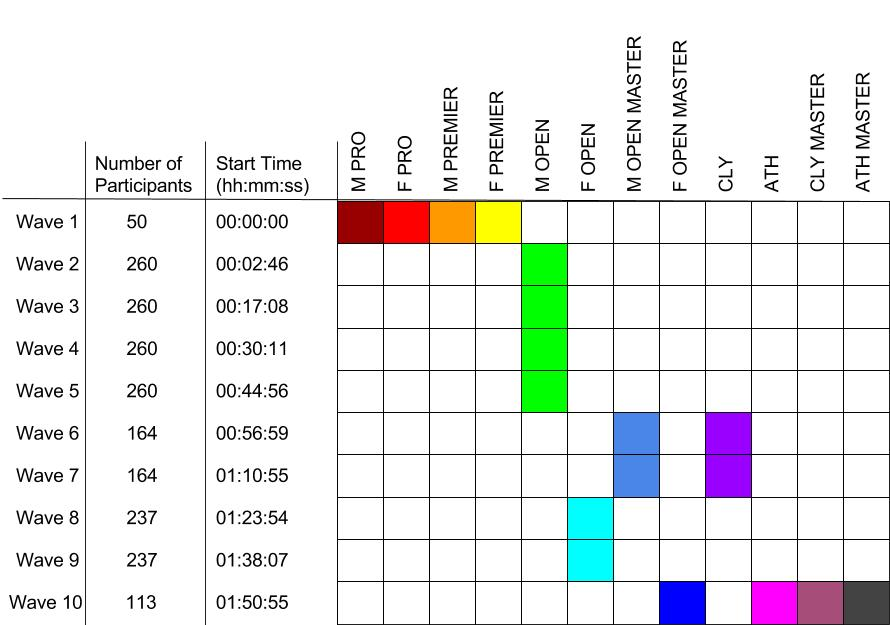
\includegraphics[width=1\textwidth]{Diagram.jpg}
  \caption{A complete schedule based on our model.}
\end{figure}
\clearpage

\clearpage
\tableofcontents
\clearpage
\section{Introduction}
\subsection{Problem}
Triathlons are a sequential group of demanding athletic events. The events are most often a long distance form of swimming, road-cycling, and running, generally in that order and with transitions between consecutive events. Transitions are time to change gear from one event to another. The participants are ranked on achievement in terms of time; the lower the time the higher ranked a race participant is. The total time is started when they first begin swimming and ends when they finish the run or equivalent final event.\par{}
These events often have a large variance in achievement, due to the various fitness backgrounds of participants. This has potential to cause unpleasantness for both the more competitive triathletes and the amateur triathletes. These complaints come from bad planning and timing that leads to congestion on the course. To mitigate congestion without extending the race to an unrealistic duration, it is necessary to take into account duration the roads are closed, individual triathletes ability and times, and the targeted audience.

\subsection{Analysis of Problem}

This larger problem can be resolved into three base constraints that must be adhered to in order to create an optimal schedule. First, we must have a basic understanding of triathlons, and more specifically how this triathlon will be organized. We must then, because the race is open registration, separate the participants into divisions based on non-race based factors such as age, weight, sex, and triathlon experience. With this, we can use divisions and past knowledge on division performance to create starting “waves” or groups that start together at the beginning of the race. This is necessary to increase the size of smaller divisions as well as decrease the size of larger divisions.\par 

With this information we can begin to develop models to be used in mitigating the issue of congestion, while decreasing the total times the roads have to be closed for race course use. Be doing this and minimizing both as much as possible, or in the case of closing the roads closing them with as few people still racing as possible.

\section{Considerations and Constraints}
\subsection{Constraints set by Mayor}
The Mayor asks for the race be fair to the public. Amateur participants should not be negatively effected for being new to this form of athletic activity. However, they also asked the maximum time that roads can be closed is 5.5 hours. However, the time that the roads are closed should be minimized. This only includes the time from when the first racer gets out of the pool to when the last racer finishes (or as close to that as possible). The time starts when they get out of the pool to account for the time it takes to close the roads. On the finishing end of the race it may be necessary for some people to be pulled from the race in order to close the roads again.

\subsection{Constraints set by The Super Tread Race Company (Sponsorship)}
The congestion should be limited in the course. This is to increase the marketability of the race to professional and serious amateur participants.
\subsection{Road Open Length}
When determining a way to measure the total time the roads would need to be closed we found there were a few things that needed to be considered. First, the maximum time the roads can be closed ($R_{closed}$) is equal to 5.5 hours. The swimming section could be excluded from the close time of the roads, because the roads can be open while the first triathletes are swimming. This increases the separation between waves that the race can have, and considered the time it takes to close the roads by including the first transition in the road close time as setup time for the roads being closed. This we represented with,
\[R_{closed} = B + T + R\]
where $T$ is the expected time for the first transition and the second transition combined or \(T = T_1 + T_2\), $B$ is the expected time needed for the biking section, and $R$ is the expected time needed for the run. 
\par{}
The cutoffs will occur on the roads themselves. Runners and bikers are expected to get off the roads when the time limit for keeping the roads open hits.
\subsection{Definition of Course Congestion}
In determining how "congested" a race course is we had to develop a definition of "congested." The Super Tread Race Company would like for the slower athletes not to hinder the faster athletes in each category. So, our first parameter of congestion is making sure that the faster divisions start their run before the slower divisions. Our second parameter of congestion is the overlap between groups. The fastest triathlete from one group will usually be faster than the slowest triathlete from the group that started earlier. This congestion can be minimized by increasing the distance between start times of each group. The third parameter of congestion is the size of the groups themselves. There may be a group of 1000 people who have similar race times. It would not be wise to start all of them at the same time, as athletes would struggle with the congestion. So, our optimal model should have low values for all of these parameters of congestion.

Another parameter of congestion to consider is linear participator density. This is the number of triathletes in one distance at a point in time. This can be scaled from specific sections of the course up to sections of the course or even the density of the whole course. This is calculated in our computational model, and won't be considered for the analytical models.
\subsection{Definition Divisions}
When deciding what division would be best implemented we implemented a variety of separating factors to best distinguish the participating population into similar skill level groups as well as splitting the groups by information based on readily available information such as sex, weight, and age as in Table 1.  Standard separating factors do not include age, however, when analyzing data we found that after age fifty total time decrease considerably as in Figure 2.
\begin{figure}[H]
    \label{fig:Why50}
  \centering
  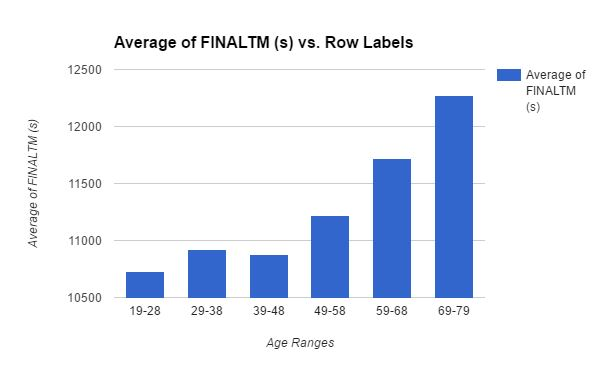
\includegraphics[width=1\textwidth]{Why50.JPG}
  \caption{Bar Graph showing the jump in Final Times after the age of 49}
\end{figure}

\begin{table}[H]
\centering

\label{Table 1}
\begin{tabular}{|l|l|l|}
\hline
\textbf{Long Name}   & \textbf{Abbreviation} & \textbf{Description}                \\ \hline
Male Professional    & M PRO        & Best male athletes in the nation and world     \\ \hline
Female Professional   & F PRO        & Best female athletes in the nation and world    \\ \hline
Male Premier      & M PREMIER      & Fastest male amateurs in previous triathlons    \\ \hline
Female Premier     & F PREMIER      & Fastest female amateurs in previous triathlons   \\ \hline
Male Open        & M OPEN        & Males under 50 years of age             \\ \hline
Female Open       & F OPEN        & Females under 50 years of age            \\ \hline
Male Open Masters    & M OPEN MASTER    & Males 50 or more years of age            \\ \hline
Female Open Masters   & F OPEN MASTER    & Females 50 or more years of age           \\ \hline
Open Clydesdale     & CLY         & Males over 220 pounds                \\ \hline
Open Athena       & ATH         & Females over 165 pounds               \\ \hline
Open Clydesdale Masters & CLY MASTER      & Males over 220 pounds and 50 or more years of age  \\ \hline
Open Athena Masters   & ATH MASTER      & Females over 165 pounds and 50 or more years of age \\ \hline
\end{tabular}
\caption{Explanation of division separations.}
\end{table}
\subsection{Determination of Waves}
To make sure there will be no congestion in the triathlon and to  These waves were decided on the basis that each starting group should start with a similar number of participants, and the waves should be grouped by similar expected skill level. We determined the maximum value for the participants in a wave to be the number of people who can stand side by side with their arms stretched out across 500m. We used 500m as the average width of the road, and we used 1.5m as the average person's wingspan [1]. So, the maximum number of people in one wave is 333.  With these considerations we were able to determine starting waves. 
\begin{table}[H]
\centering
\label{my-label}
\begin{tabular}{|l|l|l|}\hline
\textbf{Wave Number} & \textbf{Divisions in Wave}             & \textbf{Expected Participants}\\\hline
1      & M PRO, F PRO, M PREMIER, F PREMIER     & 50\\\hline
2, 3, 4, 5 & M OPEN                   & 260\\\hline
6, 7    & M OPEN MASTER, CLY             & 164\\\hline
8, 9    & F OPEN                   & 237\\\hline
10     & F OPEN MASTER, CLY MASTER, ATH, ATH MASTER & 113\\ \hline   
\end{tabular}
\caption{Starting waves were created with similar expected total times in mind. Waves that include participants from the same division (ex. 2, 3, 4, 5) are chosen by bib number.}
\end{table}
\section{General Assumptions}
\begin{itemize}
  \item \textbf{Each wave of race participants starts with a modified “Open Water” starting method.} The “Open Water” starting method characterized by the wave of participants amassing at the edge of the water before entering as a group. For use in this model we used a modified version of this starting method. In this modified “Open Water” start, the triathletes line up shoulder to shoulder on the edge of the water and begin their swim at the same moment.
  \item \textbf{The course width is constant.} If the course includes sections that are narrower or wider than others, the participator density will be affected thereby affect the speed of each racer.
  \item \textbf{No section of the triathlon course doubles back on itself or overlaps.} This is done to minimize the congestion of a single section of the course. This is necessary because an overlap would increase the participator density by a factor equal to the number of sections of the course that are overlapping. Having said this, the course could run two directions on opposite sides of the road as long as the width is kept constant throughout the track.
  \item \textbf{The roads of the town can stay open during the first swim.} We allow for time to close the roads during the first transition, and roads can be opened instantaneously when the final racer is finished. This eliminates the need for roads to be closed for the whole race, and makes sense as the roads do not take a long time to close as it would only require cars to clear out and barriers to be put up. Similarly, opening roads would be as simple as removing barriers.
  \item \textbf{The given data about the previous triathlon will very closely resemble the triathlon we are conducting.} This is important because all of our calculations are using the data from the previous triathlon. Since the sample size of runners is so huge, the data should be representative of the average triathlon.
\end{itemize}
\section{First Analytical Model}
\subsection{Variables and Variable Determination}
\(S_{n}\) = the starting time of the group n relative to when the roads open\vspace{2ex} \par \noindent 
\(S_n^{fast}\) = the starting time of the fastest swimmer in group n relative to when the roads open\vspace{2ex} \par \noindent 
\(T_1\) = transition time for the transition between the swim and the bike\vspace{2ex} \par \noindent
\(t_n^{slow}\) = the time it takes the slowest swimmer in group n to complete the swimming section (time starts when swimmer begins swimming)\vspace{2ex} \par \noindent
\(t_n^{fast}\) = the time it takes for the fastest person in the nth section to complete the swimming portion\par \vspace{2ex}

When determining these values for these variables, we used performance results from triathlons past for each division, then manipulated this data to fit the ten starting waves of participants that we deemed necessary to pass almost all participants through the course. With these new smaller data sets, we took the fastest and slowest swim times from these waves and employed those in our model. Similarly, we employed the same technique to find other values in this model. 
\subsection{Construction of Analytical Model}
To start with, we made our model without placing too much consideration on the time limit placed on the triathlon by the mayor. We tried to find the wave start times that would result in the least congestion. Our goal was to have the fastest triathlete from one group to not interact with the slowest triathlete in the group ahead until after the first transition area.
\subsection{Results}
To minimize congestion, there needed to be no overlap in waves during the swimming and first transition. First, it needs to be noted that the road closure time starts only as the first person gets out of the pool. This can be represented by:
\[S_0 = 0 - S_0^{fast}\]\
Then, to determine the starting value of waves one through nine, we first determined that a wave, which is determined by participants speed, must start in the correct consecutive place.
\[S_{n} >= S_{n-1}\]
having determined this, we also considered that if the time in the pool and transition area was not to include passing between two waves then,
\[S_n - S_{n-1} = t_{n-1}^{slow} + T_1 - t_n^{fast}\]
therefore,
\[S_n = S_{n-1} + t_{n-1}^{slow} + T_1 - t_n^{fast}\]
With this equation we can input values for each respective wave of a participants and then find when they start. We used Excel to derive the values for each of our variables, and put them in this table: \par

\begin{table}[H]
\centering

\label{my-label}
\begin{tabular}{|c|c|}
\hline
Wave \# & Start Times (seconds after roads close) \\\hline
Wave 1  & -913                                    \\\hline
Wave 2  & -236                                    \\\hline
Wave 3  & 2913                                    \\\hline
Wave 4  & 6062                                    \\\hline
Wave 5  & 9184                                    \\\hline
Wave 6  & 11762                                   \\\hline
Wave 7  & 14419                                   \\\hline
Wave 8  & 17076                                   \\\hline
Wave 9  & 19176                                   \\\hline
Wave 10 & 20992                                   \\\hline

\end{tabular}
\caption{Start Times for Each Wave}
\end{table}

With this we found that the second wave starts around 10 minutes after the first, and the separation between waves gets much larger after each group, as the slowest time gets slower after each wave. The separation between wave one and 10 is more than 5.5 hours.

\subsection{Implications}
We were expecting to have to disqualify some athletes for being too slow and making it so that the roads would have to be closed for more than 5.5 hours. However, this model makes it so that all of wave 9 and most of waves 7 and 8 would be disqualified. This does not even give these athletes a chance. As the Mayor requested we make it fun for amateur participants, and we would be cutting off participants from the CLY MASTER, ATH, ATH MASTER, and F OPEN MASTER divisions.\par{}
This model also has each of the waves 
This model aimed at minimizing congestion in the pool by not allowing waves of participants overlap early in the race, the faster from one group would not reach the slower from the group ahead of them. By doing this, it became evident that a new form of wave organization or some overlap was required. A new model would have to increase congestion to make sure more triathletes can finish the race.
\subsection{Model Assessment}
\subsubsection*{Strengths}
  This model is strong in that it gives a large cushion for each wave, which reduces overlap due to triathletes that perform outside of their expected division level. Similarly, because congestion is minimized at the beginning the average congestion for the whole race is only affected by the range of racer speeds in the biking, second transition and running sections of the race. Congestion is limited because each of the three parameters of congestion is minimized. Finally, and most importantly, this provides a base model that we can adjust to come up with a better solution.
\subsubsection*{Weaknesses}
  The most evident weakness in this model is total time. Using the slowest possible person from each group makes the start time for each group far too high. In turn this makes the total open road time much greater than the requested maximum of 5.5 hours. Many people are not even given a chance to participate, which means we would not be catering to or even permitting some amateur triathletes.
  
\section{Improved Analytical Model}
\subsection{Variables and Variable Determination}
\(S_{n}\) = the starting time of the group $n$ relative to when the roads open\vspace{2ex} \par \noindent 
\(S_n^{lower}\) = the starting time of the person who is slower than only 0.25 of the wave in wave $n$ relative to when the roads open\vspace{2ex} \par \noindent 
\(T_1\) = transition time for the transition between the swim and the bike\vspace{2ex} \par \noindent
\(t_n^{upper}\) = the time of the swim section of the person who is slower than 0.75 of the group $n$. Section (time starts when swimmer begins swimming)\vspace{2ex} \par \noindent
\(t_n^{lower}\) = the time it takes for the person who is slower than only 0.25 of the wave in the $n$th wave to complete the swimming portion\par \vspace{2ex}
\noindent
The only variable that is different from the original model is $t_n^{upper}$. This value is used instead of the time of the slowest racer, to fit all the starting times in the given 5.5 hours.
\subsection{Construction of Model}
This model is very similar to the other model, but we are changing the value that represents a slow racer from a group. Using the slowest racer for this value results in a large number of people unable to compete in the race. Using the triathlete that is slower than 75\% of the participants of triathletes and faster than 25\% of triathletes solved this problem, as this will make the starting time of each wave closer to t = 0. Also, this makes it so that the contributors to congestion are outliers of a wave. So, there will never be a large crowd of athletes overtaking another crowd of athletes.
\subsection{Results}
Again, we were trying to minimize was the starting time for each individual wave while also minimizing congestion. Because the roads only close when first swimmer is expected to finish, the first wave's start time relative to the closing of the roads can be found with,
\[S_0 = 0 - S_0^{lower}\]
Then, as in the previous model, to determine the starting value of waves one through nine, we first determined that a wave, which is determined by participants speed, must start in the correct consecutive place.
\[S_{n} >= S_{n-1}\]
with this, we also considered that if the time in the pool and transition area was not to include passing between two waves then,
\[S_n - S_{n-1} = t_{n-1}^{upper} + T_1 - t_n^{lower}\]
therefor,
\[S_n = S_{n-1} + t_{n-1}^{upper} + T_1 - t_n^{lower}\]

With this new iteration of the model we found that we could minimize expected congestion and still fit most of the participants within the five hour window.

We confidently predict that 75\% of triathletes from all waves will be able to finish the race, and 90\% of the triathletes from all waves except wave 8,9, and 10 will be able to finish the race despite the constraint that we will only be able to keep the roads closed for 5.5 hours. These results are summarized in the table below:

\begin{table}[H]
\centering
\label{my-label}
\begin{tabular}{|c|c|c|}
\hline
Wave    & T by which 75\% of the Wave will Finish & T By Which 90\% of the Wave will Finish \\\hline
 1  & 2:05:25                                         & 2:14:12                                         \\\hline
 2  & 2:57:48                                         & 3:19:55                                         \\\hline
 3  & 3:13:49                                         & 3:15:52                                         \\\hline
 4  & 3:23:41                                         & 4:03:17                                         \\\hline
 5  & 3:40:33                                         & 4:26:50                                         \\\hline
 6  & 4:03:47                                         & 4:57:23                                         \\\hline
 7  & 4:17:54                                         & 5:18:16                                         \\\hline
 8  & 4:45:06                                         & \textbf{5:45:22}                                \\\hline
 9  & 4:55:01                                         & \textbf{6:03:45}                                \\\hline
 10 & 5:26:34                                         & \textbf{6:43:00}                                \\\hline
\end{tabular}
\caption{Our predictions for the time by which 75\%  and 90 \% of the triathletes in each wave will finish the race. The waves who will have some non-finishers due to the constraints for a maximum road closure time of 5.5 hours are in bold.}
\end{table}

\begin{table}[]
\centering

\label{my-label}
\begin{tabularx}{17cm}{|C|C|C|}
\hline
Wave & Start Time Relative to Road Closure Time (Seconds) & Start Time Relative to Race Start (Seconds) \\ \hline
1  & -913 & 0\\ \hline
2  & -747 & 166\\ \hline
3  & 115 & 1028\\ \hline
4  & 898 & 1811\\ \hline
5  & 1783 & 2696\\ \hline
6  & 2506 & 3419\\ \hline
7  & 3342 & 4255\\ \hline
8  & 4121 & 5034\\ \hline
9  & 4974 & 5887\\ \hline
10  & 5742 & 6655\\ \hline
\end{tabularx}
\caption{Summary of start times based on the second analytical model we developed}
\end{table}

\subsection{Implications}
This model gives us a time to start each wave based on the upper and lower quartiles of each starting wave of participants. This allows us to build a schedule of start times that minimize congestion on the course as well as allow participants ample time to complete the course. When the fastest racer from one group reaches the first transition zone, only 0.25 of the previous group will remain in the Swim and first transition areas. Therefore, overtaking and congestion is minimized, and fast triathletes in all waves can comfortably race. Some of the slower triathletes in Wave 9 and 10 will not be able to finish the race, as the roads will open up again. We were anticipating this would happen, as some triathletes spend more than 5.5 hours on the roads.

\subsection{Model Assessment}
\subsubsection*{Strengths}
This model for scheduling has a distinct benefit of ignoring outliers, where the outliers would dramatically effect the results as in the previous model. The new start times are much more reasonable. There is now ample time between the sections for each wave to get ready, and the last wave starts with enough time for the average racer to finish. So, with this model, the average racer from each group will finish the race. This model also limits congestion because the three parameters of congestion are limited.
\subsubsection*{Weaknesses}
The weakness of the model is that some people are required still required to stop the race before finishing. This was expected however, we believe that some people who are cut would be able to finish the race given they start in an earlier wave. For example, let’s compare two slow runners from the F OPEN Young category and the Athena category. If both runners race a 4.2 hour triathlon, the woman running in the Athena category does not get to finish because of the time limit. However, the woman running in the F OPEN category gets to finish the race. Unfortunately, no matter how we arrange the divisions, one group will be but in an unfair situation. This problem can only be avoided by putting the Pros and Premiers in Wave 10, but this would severely elevate congestion, which is a value we are trying to keep as low as possible. This would be unpleasant to find out as an amateur racer, however, we rationalized this as if we placed slower people in earlier waves, the congestion would increase thereby decreasing the satisfaction of the race sponsors. By not allowing a few people to finish, we are able to moderately please both the mayor and the sponsorship that are supporting the race and if we move the participants who are not scheduled to finish forward in a wave, the sponsorship would be displeased and possibly not support the race in the future. This model is also 

\section{Computational Model}

\subsection{Addendum to General Assumptions Specific to Computational Model}
\begin{itemize}
  \item \textbf{The course can be represented linearly.} This is essential for model simplicity. In terms of real world utilization, passing is still possible because the agents in our models do not undergo collisions.
  \item \textbf{The area of the transition space will not change dramatically enough to make a major impact on total time.} We are not given an area for the calculation of density in the transitional area. We represented it with one patch, and used a velocity that kept time consistent with given data.
\end{itemize}

\subsection{Design}
In designing a computational model we further developed our measurement of congestion through the race. We were able to to measure this through the development of an agent-based model using NetLogo. In this model we constructed a triathlon course that fit both the expectations of the triathlon and our assumptions. First, the spawn point of the turtles and the swim stretch are generated, then the first half of the transition area (representing T1). Next, the biking section that does not double back or overlap itself is plotted. The second section of the transition area (representing T2) and the run loop that also does not overlap itself is also plotted. This was done by coloring a standard unit in NetLogo: patches. Each section was colored a different color in order to distinguish the sections as well as to help with agent AI modeling. \par

Once patches were created, we spawned turtles, the agents of our model. In doing this we assigned turtle to respective divisions (M Pro, F Premier, etc.) based on the previous separation of participants. The behavior of the turtle is governed both by the patch that is resides upon and its.

\begin{figure}[H]
\label{fig:racecourse}
  \centering
  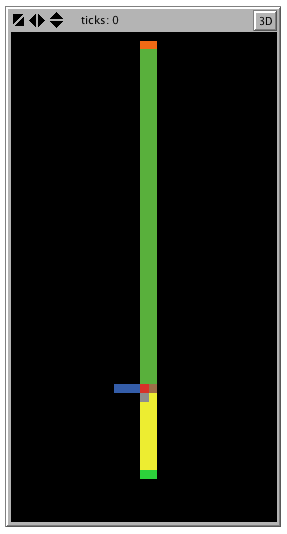
\includegraphics[width=0.25\textwidth]{RaceCourse}
  \caption{A depiction of the racecourse designed in NetLogo.}
\end{figure}

\begin{table}[H]
\centering

\label{tab:colors}
\begin{tabular}{|p{2.5cm}|p{2.5cm}|p{10cm}|}
\hline
\textbf{Race Section} & \textbf{Patch Color} & \textbf{Turtle Behavior}\\ \hline
Swim         & Blue         & Move forward at a pace representative of possible competitors swimming speed\\ \hline
Transition One    & Red         & Turn left and move forward at a pace that\par would make the turtle spend the correct average amount of time in the first transition area \\ \hline
Bicycling       & Green      & Move forward at a pace representative of \par possible competitors biking speed\\ \hline
Bicycling Turn    & Orange        & Turn right and move at the same pace as before\\ \hline
Transition Two    & Brown        & Move forward at a pace that would make the\par turtle spend the correct average amount of time in the second transition area\\ \hline
Run          & Yellow        & Move forward at a pace representative of possible\par competitors running speed\\ \hline
Run Turn       & Lime     & Turn right and move forward at a pace \par representative of possible competitors running speed\\ \hline
Finish        & Grey         & Removes oneself from model\\ \hline
\end{tabular}
\caption{Turtle behavior is based on the section of the course which it currently in; this is denoted by the patch color below it.}
\end{table}

Once this process was completed, turtles were spawned based on the devised waves and divisions from the analytical model. The number of turtles in each division was proportional to sample data set provided. Each turtle would on average move forward one patch (defined to be 500m) based on how the average time participants of the same category in the data set performed. This process was split over the entire population of varying participants who each maintained their own specific speeds. This model was also made heavy use of the benefits of the agent-based modeling approach through the use of randomization of the speeds of each turtle who as a group would perform similarly to the data set. 

This processes used a hybrid of both Microsoft Excel and NetLogo. The computationally expensive speed calculations of each category was performed in Excel and exported as a '.csv' (comma separated value list). This '.csv' was then parsed using NetLogo to obtain the speed matrix for the model. Excel was also used to calculate the wave matrix which supplied the starting times of each successive wave.

The NetLogo program was also very flexible its in initialization parameters. The program is able to take in a start and a wave division parameter for each type of participant. It is also able to vary the lengths of each of the sections of the racecourse allowing for sensitivity analysis of the racecourse congestion based on our supplied wave times and divisions.

Charts were generated throughout each model so that the density of the specific track sections could be monitored. The different types of turtles were also colored using varying shades of blue and pink to denote their specific category.

\begin{figure}[H]
\label{fig:racecourse}
  \centering
  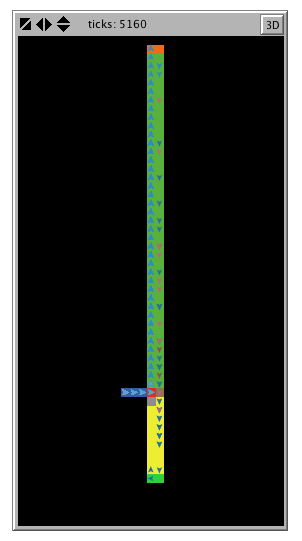
\includegraphics[width=0.25\textwidth]{RaceCourseWithTurtles}
  \caption{A depiction of the course with participants modeled on it.}
\end{figure}

\subsection{Results}
From the computational model, we can draw conclusions about the the congestion of the course at different sections. Similarly, with modification of the initial parameters we can use the computational model to compare changes in the congestion based on variations in distances of sections of the race course. Firstly, it is necessary to understand what our model predicts in terms of congestion Figure 4.

Each of the graphs represents a specific section the course using the initial length parameters given for each section of the course. Qualitatively, we can observe the peaks as each wave peaks in their population upon the section.

\begin{figure}[H]
    \label{fig:optimalCharts}
  \centering
  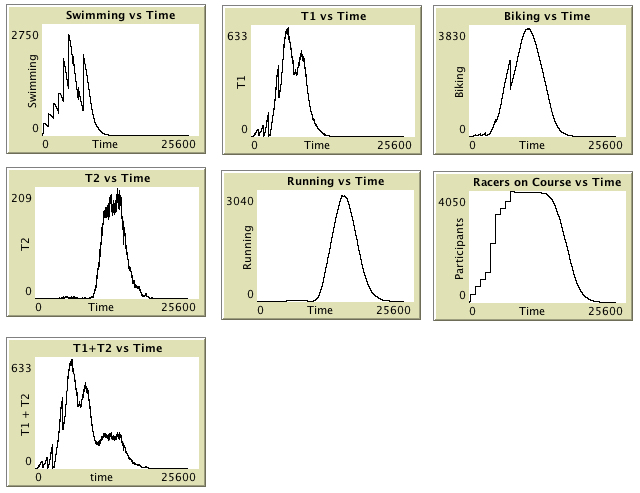
\includegraphics[width=1\textwidth]{optimalGraphs.png}
  \caption{Form the computational model we were able to collect the following graphs from one trial. The y axis is all in unit of participants, and the x axis are in units of seconds}
\end{figure}

\paragraph{Advantages in Congestion based on variation of racecourse lengths}
Through the use of NetLogo Behavior Spaces, we were able to generate a lengthy data analysis plots that allowed us to visualize the maximum linear density of the participants in each section. The behavior space analysis was set up using the wave separation of participants described above. The distances of the swimming, biking, and running portions of the course were altered amongst each other to provide for 27 different scenarios which were repeated three times a piece for increased consistency of data. 

The linear density of each section was analyzed by the following metric:

$$D_l = \frac{congestion_{max}}{distance_{section}}$$

Since Swimming is the first event its linear density is not affected by the variation of the other parts of the races' lengths. Hence its density is depicted below with the three bars representing each swim distance density. We can see that the swimming lengths currently in use are the best with further increases in length giving diminishing returns.

\begin{figure}[H]
    \label{fig:swimVariations}
  \centering
  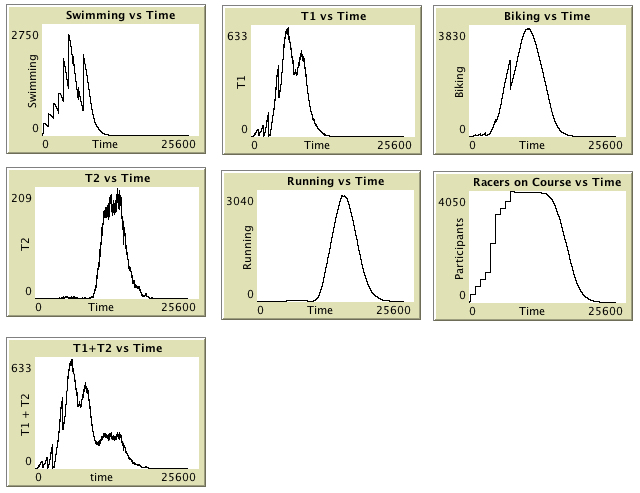
\includegraphics[width=1\textwidth]{optimalGraphs.png}
  \caption{Form the computational model we were able to collect the following graphs from one trial. The y axis is all in unit of participants, and the x axis are in units of seconds}
\end{figure}

\begin{figure}[H]
    \label{fig:Biking}
  \centering
  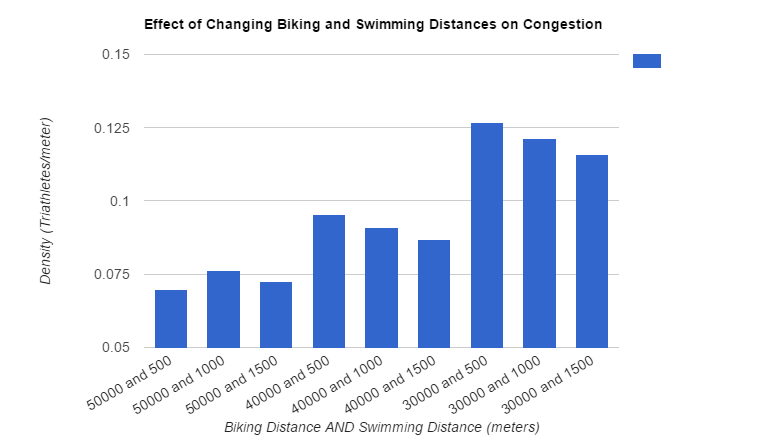
\includegraphics[width=1\textwidth]{Biking}
  \caption{This chart represents the linear density of the swimming section by length.}
\end{figure}

Analysis of the 9 bars seen in the cycling charts shown above is seen to show the variance in participant density in terms of distance in swimming and biking.  Notice the irregular behavior of the data at a longer cycling distance, and the inverse correlation between the swimming distance and and density in the larger two cycling distances.
\subsection{Model Assessment}
\subsubsection*{Strengths}
The model is able to utilize and agent-based approach to derive emergent behavior from the simple rules that govern the system. Simple parameters such as the length of each section or the starting points of each wave allow for analysis of the emergent behavior of such as congestion or run time of the race. The model is also very extensible allowing for a greater number of divisions of participants into multiple categories and great control in the modeling of the distribution of a group into waves. The computational model is also quite successful in allowing for analysis over a "behavior space" such that the underlying trends of the model can be observed.
\subsubsection*{Weaknesses}
Although a computational model posses many strengths, it posses some flaws that are important to recognize when assessing its results. The model assumes that each participant (turtle) is able to proceed throughout the courses without obstruction. Additional data would need to be procured in order to determine the effect of congestion upon the course completion. Another salient weakness the model posses is the assumptions made about the transition area. It is impossible to compare the absolute linear densities of the transition areas as the distance of the transition areas is unknown. Also the model assume the structure of the triathlon racecourse based on the common structure of such courses but the course in question may need to be structured differently though this plays into the strength of the model's adaptability.
\section{Conclusions}

When organizing an event such as a triathlon there are many critical factors that need to be considered. When analyzing this specific triathlon, we kept in mind the interests of sponsoring groups and all participants, while minimizing number or registered participants that were disqualified from the race due to failing to meet the 5.5 hour road closure limitation and minimizing the congestion on the course. We determined divisions and starting waves based on of previous equivalent triathlon performance data. We then developed an analytical model that helped us determine the optimal starting times for these waves. These optimal wave times were then implemented into a computational model that allowed us to vary values such as section distance and participant speed. This computational model also allowed us to take measurements of density and congestion during the race. With this final measurements, we were able to determine that the waves we had created (with mixed groups) should be started at irregularly spaced intervals in order to both minimize both completion time and congestion.

\paragraph{Start Times}
It is recommended that the start times that were gathered with our analytical model are adhered to in order to stagger the waves of competitors such that each is given relatively an equal opportunity to complete the course. Moreover, this schedule adheres to the race sponsors request to make the race competitive for professional and serious amateur triathletes. Comparatively, the hosting town's mayor requests the race be enjoyable to the public who can participate in this open registration race. However, the mayor also asks that the roads be closed no more than 5.5 hours. Thus we recommend that each wave start at the following times after the start of the race:
\begin{itemize}
  \item 00:00:00
  \item 00:02:46
  \item 00:17:08
  \item 00:30:11
  \item 00:44:56
  \item 00:56:59
  \item 01:10:55
  \item 01:23:54
  \item 01:38:07
  \item 01:50:55
\end{itemize}

\paragraph{Cutoff}
When hosting this event, race organizers should consider two cutoffs. One at 5.5 hours after the roads are closed for anyone who happens to still be on the race course when the 5.5 hour maximum road open time is reached. Then, there should be a second cutoff that is $5.5 - R^{fast} = $. This cutoff is for cyclists. If they have not reached the second transition by this time then they will be stopped from continuing. This cutoff is total time minus the fastest expected time of a run.

\paragraph{Recommended Divisions and Waves}
Creating a high number of fair divisions is better for our triathlon, because more awards will be given out, and more people will come to the triathlon to try to win the awards. We decided it would be prudent to use all the divisions in the given data, as well as use a division based on age. We can call this group the Masters, and anybody at or above the age of 50 can be considered a Master. We used 50 because that is the age generally used by most triathlons, and there is a big drop in times at 50 as determined through our analysis of data variation by age. This is shown in the bar graph below.

\section{Acknowledgements}
We would like to note our extensive use of both the data set provided and multiple software utilities. These software utilities include Microsoft Excel, NetLogo, and Matheamtica, and Python.
\section{References}
[1] Elert, Glenn. "Size of a Human: Body Proportions." Size of a Human: Body Proportions. N.p., 2006. Web. 13 Nov. 2016. 
\noindent
\par
[2] Competitive Rules. (2014, November). Retrieved November 13, 2016, from http://www.teamusa.org/USA-Triathlon/About/Multisport/Competitive-Rules

\section{Appendix}
Relavent Code
breed [mpros mpro]         ;; male pros \\
breed [fpros fpro]         ;; female pros \\
breed [mpremiers mpremier] ;; male premiers \\
breed [fpremiers fpremier] ;; female premeirs \\
breed [ymopens ymopen]     ;; young male open \\
breed [omopens omopen]     ;; old male open \\
breed [yfopens yfopen]     ;; young female open \\
breed [ofopens ofopen]     ;; old female open \\
breed [yclys ycly]         ;; young clysdale \\
breed [oclys ocly]         ;; old clysdale \\
breed [yaths yath]         ;; young athenians \\
breed [oaths oath]         ;; old athenians \\

;; set Globals for CSV transcriber \\
;; set counters for number of waves completed \\
globals [speeds wave-intervals \\
         mpros-total fpros-total \\
         mpremiers-total fpremiers-total \\
         ymopens-total omopens-total \\
         yfopens-total ofopens-total \\
         yclys-total oclys-total \\
         yaths-total oaths-total] \\
;; setup the canvas, set global vars, and parse the CSV data, reset ticks \\
to setup
  clear-all \\
  set-globals \\
  import-speeds \\
  import-waves \\
  draw-course\\
  reset-ticks\\
  show wave-intervals\\
  show speeds
  ;; foreach [0 1 2 3 4] [show item ? item 7 speeds]
end

;; Source CSV Parser: http://complexityblog.com/blog/index.php?itemid=88
;; Start CSV Parser Methods
to-report replace-all [string1 with-string in-string]
  while [ member? string1 in-string ] [
    let index position string1 in-string
    set in-string replace-item index in-string with-string
  ] 
  report in-string
end
to import-waves
  set wave-intervals [0 166 1028 1811 2696 3419 4255 5034 5887 6655]
end
to import-speeds
  set speeds []
  file-open "speeds.csv"
  while [not file-at-end?] [
    let thisline file-read-line
    ;show thisline
    set thisline remove " " thisline
    set thisline (word "[ " (replace-all "," " " thisline) " ]")
    ;show thisline
    set speeds lput read-from-string thisline speeds
  ]
  file-close
end
;; End CSV Parser methods

;; Set global initial values
to set-globals
set mpros-total 4
set fpros-total 4
set mpremiers-total 30
set fpremiers-total 11
set ymopens-total 1037
set omopens-total 2098
set yfopens-total 473
set ofopens-total 85
set yclys-total 29
set oclys-total 8
set yaths-total 17
set oaths-total 2
end
to draw-course
  foreach n-values (swim-dist / 500) [-1 - ?] [ask patch ? 0 [set pcolor blue]] ;; swim area
  ask patch 0 0 [set pcolor red]   ;; transition area
  ask patch 1 0 [set pcolor brown] ;; go straight

  foreach but-first n-values (bike-dist / 500 / 2) [?] [ask patch 0 ? [set pcolor green]]    ;; bike forward
  foreach but-first n-values (bike-dist / 500 / 2) [?] [ask patch 1 ? [set pcolor green]]    ;; bike backward
  foreach [0 1] [ask patch ? (bike-dist / 500 / 2) [set pcolor orange]]                      ;; bike turn
  
  foreach but-first but-first n-values (run-dist / 500 / 2) [0 - ?] [ask patch 0 ? [set pcolor yellow]]    ;; run forward
  foreach but-first n-values (run-dist / 500 / 2) [0 - ?] [ask patch 1 ? [set pcolor yellow]] ;; run backward
  show but-first n-values (run-dist / 500 / 2) [0 - ?]
  
  foreach [0 1] [ask patch ? (0 - run-dist / 500 / 2) [set pcolor lime]]
  ask patch 0 -1 [set pcolor grey]
end

to set-mpros [mpros-num]
  create-mpros mpros-num
  ask mpros [
    setxy (0 - swim-dist / 500) 0
    set color 93
    set heading 90
    ]
end
to set-fpros [fpros-num]
  create-fpros fpros-num
  ask fpros [
    setxy (0 - swim-dist / 500) 0
    set color 133
    set heading 90
    ]
end
to set-ymopens [ymopens-num]
  create-ymopens ymopens-num
  ask ymopens [
    setxy (0 - swim-dist / 500) 0
    set color 95
    set heading 90
    ]
end
to set-omopens [omopens-num]
  create-omopens omopens-num
  ask omopens [
    setxy (0 - swim-dist / 500) 0
    set color 95
    set heading 90
    ]
end
to set-yfopens [yfopens-num]
  create-yfopens yfopens-num
  ask yfopens [
    setxy (0 - swim-dist / 500) 0
    set color 135
    set heading 90
    ]
end
to set-ofopens [ofopens-num]
  create-ofopens ofopens-num
  ask ofopens [
    setxy (0 - swim-dist / 500) 0
    set color 135
    set heading 90
    ]
end
to set-mpremiers [mpremiers-num]\\
  create-mpremiers mpremiers-num\\
  ask mpremiers [\\
    setxy (0 - swim-dist / 500) 0\\
    set color 94\\
    set heading 90\\
    ]\\
end\\
to set-fpremiers [fpremiers-num]\\
  create-fpremiers fpremiers-num\\
  ask fpremiers [\\
    setxy (0 - swim-dist / 500) 0\\
    set color 134\\
    set heading 90\\
    ]
end
to set-yclys [yclys-num]\\
  create-yclys yclys-num
  ask yclys [\\
    setxy (0 - swim-dist / 500) 0\\
    set color 96
    set heading 90\\
    ]\\
end
to set-oclys [oclys-num]
  create-oclys oclys-num
  ask oclys [
    setxy (0 - swim-dist / 500) 0
    set color 96
    set heading 90
    ]
end
to set-yaths [yaths-num]
  create-yaths yaths-num
  ask yaths [
    setxy (0 - swim-dist / 500) 0
    set color 136
    set heading 90
    ]
end
to set-oaths [oaths-num]
  create-oaths oaths-num
  ask oaths [
    setxy (0 - swim-dist / 500) 0
    set color 136
    set heading 90
    ]
end

to go
  ;; Wave One
  if (member? ticks sublist wave-intervals ymopens-start-wave (ymopens-start-wave + ymopens-waves-num)) [set-ymopens ymopens-total / ymopens-waves-num]
  if (member? ticks sublist wave-intervals omopens-start-wave (omopens-start-wave + omopens-waves-num)) [set-omopens omopens-total / omopens-waves-num]
  if (member? ticks sublist wave-intervals yfopens-start-wave (yfopens-start-wave + yfopens-waves-num)) [set-yfopens yfopens-total / yfopens-waves-num]
  if (member? ticks sublist wave-intervals ofopens-start-wave (ofopens-start-wave + ofopens-waves-num)) [set-ofopens ofopens-total / ofopens-waves-num]
  if (member? ticks sublist wave-intervals mpros-start-wave (mpros-start-wave + mpros-waves-num)) [set-mpros mpros-total / mpros-waves-num]
  if (member? ticks sublist wave-intervals fpros-start-wave (fpros-start-wave + fpros-waves-num)) [set-fpros fpros-total / fpros-waves-num]
  if (member? ticks sublist wave-intervals mpremiers-start-wave (mpremiers-start-wave + mpremiers-waves-num)) [set-mpremiers mpremiers-total / mpremiers-waves-num]
  if (member? ticks sublist wave-intervals fpremiers-start-wave (fpremiers-start-wave + fpremiers-waves-num)) [set-fpremiers fpremiers-total / fpremiers-waves-num]
  if (member? ticks sublist wave-intervals yclys-start-wave (yclys-start-wave + yclys-waves-num)) [set-yclys yclys-total / yclys-waves-num]
  if (member? ticks sublist wave-intervals oclys-start-wave (oclys-start-wave + oclys-waves-num)) [set-oclys oclys-total / oclys-waves-num]
  if (member? ticks sublist wave-intervals yaths-start-wave (yaths-start-wave + yaths-waves-num)) [set-yaths yaths-total / yaths-waves-num]
  if (member? ticks sublist wave-intervals oaths-start-wave (oaths-start-wave + oaths-waves-num)) [set-ymopens ymopens-total / ymopens-waves-num]
  
  ask yaths [
    ifelse pcolor = blue [if random item 0 item 0 speeds  = 0 [fd 1]] ;; swim
    [ifelse pcolor = red [if random item 1 item 0 speeds  = 0 [set heading 0 fd 1] ] ;; t1
     [ifelse pcolor = green [if random item 2 item 0 speeds  = 0 [fd 1]] ;; bike
       [ifelse pcolor = orange [if random item 2 item 0 speeds  = 0 [rt 90 fd 1 ]] ;; bike
         [ifelse pcolor = brown [if random item 3 item 0 speeds  = 0 [fd 1]] ;; t2
           [ifelse pcolor = yellow [if random item 4 item 0 speeds  = 0 [fd 1]] ;; run
             [ifelse pcolor = lime [if random item 4 item 0 speeds  = 0 [rt 90 fd 1 ]] [die]] ;; run
             ]
           ]
         ]
       ]
     ]
    ]
    ask oaths [
    ifelse pcolor = blue [if random item 0 item 1 speeds  = 0 [fd 1]] ;; swim
    [ifelse pcolor = red [if random item 1 item 1 speeds  = 0 [set heading 0 fd 1] ] ;; t1
     [ifelse pcolor = green [if random item 2 item 1 speeds  = 0 [fd 1]] ;; bike
       [ifelse pcolor = orange [if random item 2 item 1 speeds  = 0 [rt 90 fd 1 ]] ;; bike
         [ifelse pcolor = brown [if random item 3 item 1 speeds  = 0 [fd 1]] ;; t2
           [ifelse pcolor = yellow [if random item 4 item 1 speeds  = 0 [fd 1]] ;; run
             [ifelse pcolor = lime [if random item 4 item 1 speeds  = 0 [rt 90 fd 1 ]] [die]] ;; run
             ]
           ]
         ]
       ]
     ]
    ]
  ask yclys [
    ifelse pcolor = blue [if random item 0 item 2 speeds  = 0 [fd 1]] ;; swim
    [ifelse pcolor = red [if random item 1 item 2 speeds  = 0 [set heading 0 fd 1] ] ;; t1
     [ifelse pcolor = green [if random item 2 item 2 speeds  = 0 [fd 1]] ;; bike
       [ifelse pcolor = orange [if random item 2 item 2 speeds  = 0 [rt 90 fd 1 ]] ;; bike
         [ifelse pcolor = brown [if random item 3 item 2 speeds  = 0 [fd 1]] ;; t2
           [ifelse pcolor = yellow [if random item 4 item 2 speeds  = 0 [fd 1]] ;; run
             [ifelse pcolor = lime [if random item 4 item 2 speeds  = 0 [rt 90 fd 1 ]] [die]] ;; run
             ]
           ]
         ]
       ]
     ]
    ]
  ask oclys [
    ifelse pcolor = blue [if random item 0 item 3 speeds  = 0 [fd 1]] ;; swim
    [ifelse pcolor = red [if random item 1 item 3 speeds  = 0 [set heading 0 fd 1] ] ;; t1
     [ifelse pcolor = green [if random item 2 item 3 speeds  = 0 [fd 1]] ;; bike
       [ifelse pcolor = orange [if random item 2 item 3 speeds  = 0 [rt 90 fd 1 ]] ;; bike
         [ifelse pcolor = brown [if random item 3 item 3 speeds  = 0 [fd 1]] ;; t2
           [ifelse pcolor = yellow [if random item 4 item 3 speeds  = 0 [fd 1]] ;; run
             [ifelse pcolor = lime [if random item 4 item 3 speeds  = 0 [rt 90 fd 1 ]] [die]] ;; run
             ]
           ]
         ]
       ]
     ]
    ]
  ask mpremiers [
    ifelse pcolor = blue [if random item 0 item 4 speeds  = 0 [fd 1]] ;; swim
    [ifelse pcolor = red [if random item 1 item 4 speeds  = 0 [set heading 0 fd 1] ] ;; t1
     [ifelse pcolor = green [if random item 2 item 4 speeds  = 0 [fd 1]] ;; bike
       [ifelse pcolor = orange [if random item 2 item 4 speeds  = 0 [rt 90 fd 1 ]] ;; bike
         [ifelse pcolor = brown [if random item 3 item 4 speeds  = 0 [fd 1]] ;; t2
           [ifelse pcolor = yellow [if random item 4 item 4 speeds  = 0 [fd 1]] ;; run
             [ifelse pcolor = lime [if random item 4 item 4 speeds  = 0 [rt 90 fd 1 ]] [die]] ;; run
             ]
           ]
         ]
       ]
     ]
    ]
  ask fpremiers [
    ifelse pcolor = blue [if random item 0 item 5 speeds  = 0 [fd 1]] ;; swim
    [ifelse pcolor = red [if random item 1 item 5 speeds  = 0 [set heading 0 fd 1] ] ;; t1
     [ifelse pcolor = green [if random item 2 item 5 speeds  = 0 [fd 1]] ;; bike
       [ifelse pcolor = orange [if random item 2 item 5 speeds  = 0 [rt 90 fd 1 ]] ;; bike
         [ifelse pcolor = brown [if random item 3 item 5 speeds  = 0 [fd 1]] ;; t2
           [ifelse pcolor = yellow [if random item 4 item 5 speeds  = 0 [fd 1]] ;; run
             [ifelse pcolor = lime [if random item 4 item 5 speeds  = 0 [rt 90 fd 1 ]] [die]] ;; run
             ]
           ]
         ]
       ]
     ]
    ]
  ask mpros [
    ifelse pcolor = blue [if random item 0 item 6 speeds  = 0 [fd 1]] ;; swim
    [ifelse pcolor = red [if random item 1 item 6 speeds  = 0 [set heading 0 fd 1] ] ;; t1
     [ifelse pcolor = green [if random item 2 item 6 speeds  = 0 [fd 1]] ;; bike
       [ifelse pcolor = orange [if random item 2 item 6 speeds  = 0 [rt 90 fd 1 ]] ;; bike
         [ifelse pcolor = brown [if random item 3 item 6 speeds  = 0 [fd 1]] ;; t2
           [ifelse pcolor = yellow [if random item 4 item 6 speeds  = 0 [fd 1]] ;; run
             [ifelse pcolor = lime [if random item 4 item 6 speeds  = 0 [rt 90 fd 1 ]] 
               [if random item 4 item 7 speeds  = 0 [die]]] ;; run
             ]
           ]
         ]
       ]
     ]
    ]
  ask fpros [
    ifelse pcolor = blue [if random item 0 item 7 speeds  = 0 [fd 1]] ;; swim
    [ifelse pcolor = red [if random item 1 item 7 speeds  = 0 [set heading 0 fd 1] ] ;; t1
     [ifelse pcolor = green [if random item 2 item 7 speeds  = 0 [fd 1]] ;; bike
       [ifelse pcolor = orange [if random item 2 item 7 speeds  = 0 [rt 90 fd 1 ]] ;; bike
         [ifelse pcolor = brown [if random item 3 item 7 speeds  = 0 [fd 1]] ;; t2
           [ifelse pcolor = yellow [if random item 4 item 7 speeds  = 0 [fd 1]] ;; run
             [ifelse pcolor = lime [if random item 4 item 7 speeds  = 0 [rt 90 fd 1 ]] 
               [if random item 4 item 7 speeds  = 0 [die]]] ;; run
             ]
           ]
         ]
       ]
     ]
    ]
  ask ymopens [
    ifelse pcolor = blue [if random item 0 item 8 speeds  = 0 [fd 1]] ;; swim
    [ifelse pcolor = red [if random item 1 item 8 speeds  = 0 [set heading 0 fd 1] ] ;; t1
     [ifelse pcolor = green [if random item 2 item 8 speeds  = 0 [fd 1]] ;; bike
       [ifelse pcolor = orange [if random item 2 item 8 speeds  = 0 [rt 90 fd 1 ]] ;; bike
         [ifelse pcolor = brown [if random item 3 item 8 speeds  = 0 [fd 1]] ;; t2
           [ifelse pcolor = yellow [if random item 4 item 8 speeds  = 0 [fd 1]] ;; run
             [ifelse pcolor = lime [if random item 4 item 8 speeds  = 0 [rt 90 fd 1 ]] [die]] ;; run
             ]
           ]
         ]
       ]
     ]
    ]
  ask omopens [
    ifelse pcolor = blue [if random item 0 item 9 speeds  = 0 [fd 1]] ;; swim
    [ifelse pcolor = red [if random item 1 item 9 speeds  = 0 [set heading 0 fd 1] ] ;; t1
     [ifelse pcolor = green [if random item 2 item 9 speeds  = 0 [fd 1]] ;; bike
       [ifelse pcolor = orange [if random item 2 item 9 speeds  = 0 [rt 90 fd 1 ]] ;; bike
         [ifelse pcolor = brown [if random item 3 item 9 speeds  = 0 [fd 1]] ;; t2
           [ifelse pcolor = yellow [if random item 4 item 9 speeds  = 0 [fd 1]] ;; run
             [ifelse pcolor = lime [if random item 4 item 9 speeds  = 0 [rt 90 fd 1 ]] [die]] ;; run
             ]
           ]
         ]
       ]
     ]
    ]
  ask yfopens [
    ifelse pcolor = blue [if random item 0 item 2 speeds  = 0 [fd 1]] ;; swim
    [ifelse pcolor = red [if random item 1 item 2 speeds  = 0 [set heading 0 fd 1] ] ;; t1
     [ifelse pcolor = green [if random item 2 item 2 speeds  = 0 [fd 1]] ;; bike
       [ifelse pcolor = orange [if random item 2 item 2 speeds  = 0 [rt 90 fd 1 ]] ;; bike
         [ifelse pcolor = brown [if random item 3 item 2 speeds  = 0 [fd 1]] ;; t2
           [ifelse pcolor = yellow [if random item 4 item 2 speeds  = 0 [fd 1]] ;; run
             [ifelse pcolor = lime [if random item 4 item 2 speeds  = 0 [rt 90 fd 1 ]] [die]] ;; run
             ]
           ]
         ]
       ]
     ]
    ]
  ask ofopens [
    ifelse pcolor = blue [if random item 0 item 2 speeds  = 0 [fd 1]] ;; swim
    [ifelse pcolor = red [if random item 1 item 2 speeds  = 0 [set heading 0 fd 1] ] ;; t1
     [ifelse pcolor = green [if random item 2 item 2 speeds  = 0 [fd 1]] ;; bike
       [ifelse pcolor = orange [if random item 2 item 2 speeds  = 0 [rt 90 fd 1 ]] ;; bike
         [ifelse pcolor = brown [if random item 3 item 2 speeds  = 0 [fd 1]] ;; t2
           [ifelse pcolor = yellow [if random item 4 item 2 speeds  = 0 [fd 1]] ;; run
             [ifelse pcolor = lime [if random item 4 item 2 speeds  = 0 [rt 90 fd 1 ]] [die]] ;; run
             ]
           ]
         ]
       ]
     ]
    ]

  if not any? turtles [ stop ]
  tick
end

\end{document}